\documentclass[12pt,a4paper]{article}
\usepackage[UTF8]{ctex}
\usepackage{geometry}
\geometry{left=2.5cm, right=2.5cm, top=2.8cm, bottom=2.5cm}
\usepackage{amsmath,amssymb,amsfonts}
\usepackage{graphicx}
\usepackage{booktabs}
\usepackage{multirow}
\usepackage{caption}
\usepackage{subcaption}
\usepackage{float}
\usepackage{enumitem}
\usepackage{algorithm}
\usepackage{algorithmic}
\usepackage{hyperref}
\usepackage{tabularx}
\usepackage{array}
\usepackage{longtable}
\usepackage{setspace}
\usepackage{fancyhdr}
\usepackage{titlesec}
\usepackage{appendix}

\hypersetup{colorlinks=true, linkcolor=blue, citecolor=blue, urlcolor=blue}

\pagestyle{fancy}
\fancyhf{}
\fancyhead[C]{\small 城市交通网络健壮性分析与提升策略}
\fancyfoot[C]{\thepage}

\titleformat{\section}{\Large\bfseries\centering}{\thesection}{1em}{}
\titleformat{\subsection}{\large\bfseries}{\thesubsection}{1em}{}

\renewcommand{\abstractname}{\Large\textbf{摘\quad 要}}

\begin{document}

\begin{center}
{\LARGE\bfseries 城市交通网络健壮性分析与提升策略}\\[1.5em]
\end{center}

% ==================== 摘要 ====================
\begin{abstract}
\setlength{\parindent}{2em}

本文针对8个中国城市（沈阳、大连、郑州、青岛、哈尔滨、东莞、成都、泉州）的OpenStreetMap道路网络数据，系统构建了城市交通网络图模型，从拓扑统计、随机故障、蓄意攻击、空间级联故障四个维度量化评估了网络健壮性，并设计了基于桥边消除与介数旁路的贪心加边策略以提升脆弱城市的抗攻击能力。

\textbf{针对问题一}，构建了8个城市的无向加权交通网络图，计算了节点数、边数、平均度、聚类系数、连通分量比例、直径和平均路径长等关键指标。对度分布分别进行了幂律、指数和泊松分布拟合，以$R^2$为判别标准。结果表明，8个城市的度分布均最优拟合为\textbf{泊松分布}（$R^2 \in [0.56, 0.70]$），说明这些交通网络具有均匀随机图特征，而非无标度网络。

\textbf{针对问题二}，建立了基于Molloy-Reed渗流理论的随机故障模型，通过10次蒙特卡罗模拟求取最大连通分量比率$\text{LCC}/N_0$的演化曲线，定义健壮性指标$R=\int_0^1 S(p)\,dp$。结果显示沈阳健壮性最高（$R=0.2213$），大连最低（$R=0.1510$）。理论渗流阈值$f_c$与实测临界比例吻合良好。

\textbf{针对问题三}，设计了自适应介数中心性攻击算法（HBA），以动态重计算的介数值确定最优攻击序列，并与静态度攻击和随机攻击作对比。HBA攻击效力比随机攻击高5--12倍。在HBA攻击下，\textbf{沈阳}健壮性最高（$R_{\text{HBA}}=0.0972$），大连最低（$R_{\text{HBA}}=0.0492$）。

\textbf{针对问题四}，引入空间级联故障模型，将节点失效的影响扩展到地理半径$r$内的所有节点。在$r \in \{0, 500, 1000, 2000, 5000\}$米下进行实验。结果表明，随着波及半径增大，单次攻击移除的节点数增加，以节点比例为x轴的健壮性$R$反而增大（$r=0$时$R\approx 0.10$，$r=5000$m时$R\approx 0.40$），这是因为批量移除降低了攻击精度。

\textbf{针对问题五}，以沈阳（$R_{\text{HBA}}=0.0972$）为目标基准，设计了融合桥边消除与介数旁路的贪心加边策略，在200条边的预算约束下为7个城市生成了具体的加边方案。泉州仅需80条边即接近目标；其余城市在200条边预算内虽未完全达标，但均实现了显著的健壮性提升。

\vspace{0.5em}
\noindent\textbf{关键词：}交通网络；网络健壮性；渗流理论；介数中心性攻击；空间级联故障；贪心加边优化
\end{abstract}

\newpage
\tableofcontents
\newpage

% ==================== 一、问题重述 ====================
\section{问题重述}

\subsection{问题背景}

城市交通网络作为城市运行的核心基础设施，其健壮性直接关系到城市在面对自然灾害、设备故障或蓄意破坏时的韧性能力。随着城市化进程加速，理解交通网络的拓扑脆弱性并提出有效的增强策略，已成为城市规划与应急管理中的关键科学问题。

本题提供了8个中国城市（沈阳、大连、郑州、青岛、哈尔滨、东莞、成都、泉州）基于OpenStreetMap的交通网络边列表数据，要求依次解决以下五个问题：

\subsection{问题概述}

\begin{enumerate}[label=\textbf{问题\arabic*：}, leftmargin=4em]
    \item 构建城市交通网络图，计算基本拓扑统计量（聚类系数、直径、度分布等），并使用数学模型拟合度分布。
    \item 利用渗流理论评估随机节点故障下的网络健壮性，计算临界故障比例，识别网络性能急剧下降的阈值。
    \item 设计最优蓄意攻击策略，找到使网络健壮性最低的节点移除序列，对比不同攻击策略的效力，确定健壮性最高的城市。
    \item 建立空间级联故障模型，考虑节点失效波及一定地理半径内所有节点的情形，分析不同半径对网络存活能力的影响。
    \item 提出新增边策略提升脆弱城市的网络健壮性，以最小建设成本使其达到最健壮城市的水平。
\end{enumerate}

% ==================== 二、问题分析 ====================
\section{问题分析}

\subsection{问题一的分析}

问题一要求从原始边列表数据中构建城市交通网络图，并提取关键拓扑特征。核心在于：（1）正确处理数据中的节点坐标与边权信息；（2）计算包括聚类系数、直径、连通分量等在内的网络统计量；（3）采用幂律分布$P(k)\sim k^{-\gamma}$、指数分布$P(k)\sim e^{-\lambda k}$和泊松分布$P(k)=\frac{\langle k\rangle^k e^{-\langle k\rangle}}{k!}$三种经典模型对度分布进行拟合。度分布的类型决定了网络的基本类别——无标度网络对蓄意攻击脆弱而对随机故障健壮，而泊松型网络的行为则更为均匀。

\subsection{问题二的分析}

问题二的核心是评估网络在随机失效下的退化过程。我们采用Molloy-Reed准则计算理论渗流阈值$f_c = 1 - \frac{1}{\kappa - 1}$（其中$\kappa = \langle k^2 \rangle / \langle k \rangle$），并通过蒙特卡罗模拟获得经验健壮性曲线。关键指标包括：健壮性积分$R$、50\%连通性丧失对应的临界比例$p_{0.5}$、以及最大下降速率点$p^*$。

\subsection{问题三的分析}

问题三要求找到使网络最快瓦解的攻击策略。已有研究表明，基于介数中心性的自适应攻击（HBA）是最具破坏力的攻击方式之一。其原理在于：介数中心性高的节点承载了大量最短路径流量，移除后会导致路径重组和网络碎片化。为提高算法效率，采用近似介数计算与分批重算策略。

\subsection{问题四的分析}

问题四引入了空间维度，将单节点失效扩展为地理区域失效。这模拟了自然灾害（如地震、洪水）等空间相关性失效场景。需要建立kd-tree空间索引以高效查询邻域节点，并在不同波及半径$r$下分析网络退化规律。

\subsection{问题五的分析}

问题五是一个网络优化问题，需要在成本约束下通过添加新边来提升网络健壮性。关键挑战在于：（1）候选边空间极大（$O(N^2)$），需要高效的启发式筛选；（2）健壮性评估计算代价高，需要代理指标加速优化循环。我们采用桥边消除与介数旁路两种策略生成候选边，并用贪心算法逐步添加。

% ==================== 三、模型假设与符号说明 ====================
\section{模型假设与符号说明}

\subsection{模型假设}

\begin{enumerate}[label=\textbf{假设\arabic*：}, leftmargin=4em]
    \item 交通网络建模为无向图，即道路为双向通行。
    \item 边权为道路的欧氏长度（单位：米），节点坐标忠实反映地理位置。
    \item 网络连通性以最大连通分量（LCC）占初始节点数的比例衡量。
    \item 随机故障中各节点独立等概率失效，不考虑节点间的相关性。
    \item 空间级联故障中，波及半径$r$内的所有节点同步失效。
    \item 新增道路的建设成本与其欧氏距离成正比。
    \item 在问题五中，不考虑地形、政策等非拓扑约束。
\end{enumerate}

\subsection{符号说明}

\begin{table}[H]
\centering
\caption{主要符号说明}
\begin{tabular}{cl}
\toprule
\textbf{符号} & \textbf{含义} \\
\midrule
$G=(V,E)$ & 交通网络图，$V$为节点集，$E$为边集 \\
$N=|V|$ & 网络节点数 \\
$M=|E|$ & 网络边数 \\
$\langle k \rangle$ & 平均度 \\
$C$ & 平均聚类系数 \\
$\kappa$ & 度分布的二阶矩与一阶矩之比，$\kappa = \langle k^2 \rangle / \langle k \rangle$ \\
$f_c$ & Molloy-Reed理论渗流阈值 \\
$p$ & 节点移除比例 \\
$S(p)$ & 移除比例为$p$时的LCC$/N_0$比率 \\
$R$ & 健壮性指标，$R = \int_0^1 S(p)\,dp$ \\
$r$ & 空间级联故障的波及半径（米） \\
$B_C(v)$ & 节点$v$的介数中心性 \\
\bottomrule
\end{tabular}
\end{table}

% ==================== 四、模型建立与求解 ====================
\section{模型建立与求解}

\subsection{问题一：网络拓扑特征分析与度分布建模}

\subsubsection{网络构建}

由CSV边列表数据构建无向加权图$G=(V,E)$：每条记录包含起点\texttt{START\_NODE}、终点\texttt{END\_NODE}、边长\texttt{LENGTH}及节点坐标\texttt{(XCoord, YCoord)}。将所有边加入图中，边权取道路长度。

\subsubsection{基本统计量计算}

对每个城市的交通网络，计算如下统计量：

\begin{itemize}[leftmargin=2em]
    \item \textbf{平均度}：$\langle k \rangle = \frac{2M}{N}$
    \item \textbf{平均聚类系数}：$C = \frac{1}{N}\sum_{v \in V} C_v$，其中$C_v = \frac{2T_v}{k_v(k_v - 1)}$，$T_v$为节点$v$邻居间的三角形数
    \item \textbf{最大连通分量占比}：$\text{GCC} = |V_{\text{LCC}}| / N$
    \item \textbf{直径与平均路径长}：采用抽样法（80个随机源节点）估计，取99分位数为直径估计
\end{itemize}

\subsubsection{度分布拟合模型}

分别采用三种分布模型进行非线性最小二乘拟合（\texttt{scipy.optimize.curve\_fit}）：

\begin{enumerate}[label=(\arabic*)]
    \item \textbf{幂律分布}：$P(k) = C \cdot k^{-\gamma}$，参数为$C$和$\gamma$
    \item \textbf{指数分布}：$P(k) = C \cdot e^{-\lambda k}$，参数为$C$和$\lambda$
    \item \textbf{泊松分布}：$P(k) = \frac{\langle k \rangle^k e^{-\langle k \rangle}}{k!}$，参数为$\langle k \rangle$（取实测均值）
\end{enumerate}

以$R^2 = 1 - \frac{\sum(y_i - \hat{y}_i)^2}{\sum(y_i - \bar{y})^2}$为拟合优度判别标准。

\subsubsection{结果与分析}

\begin{table}[H]
\centering
\caption{8个城市交通网络基本拓扑统计量}
\resizebox{\textwidth}{!}{
\begin{tabular}{lrrrrrrrrrr}
\toprule
\textbf{城市} & $N$ & $M$ & $\langle k \rangle$ & $k_{\max}$ & $C$ & \textbf{分量数} & \textbf{GCC占比} & \textbf{直径} & \textbf{路径长} & \textbf{最优$R^2$} \\
\midrule
沈阳 & 13000 & 19026 & 2.927 & 14 & 0.0509 & 59 & 0.9808 & 80 & 41.46 & 0.5679 \\
大连 & 13605 & 17897 & 2.631 & 7 & 0.0459 & 390 & 0.9092 & 151 & 72.82 & 0.5605 \\
郑州 & 9162 & 12865 & 2.808 & 8 & 0.0306 & 25 & 0.9808 & 80 & 41.33 & 0.6194 \\
青岛 & 13894 & 19018 & 2.738 & 8 & 0.0301 & 211 & 0.9526 & 138 & 64.68 & 0.6468 \\
哈尔滨 & 10727 & 14711 & 2.743 & 7 & 0.0397 & 131 & 0.9445 & 128 & 52.99 & 0.5616 \\
东莞 & 8315 & 11128 & 2.677 & 7 & 0.0362 & 130 & 0.9210 & 102 & 45.76 & 0.5978 \\
成都 & 18300 & 25930 & 2.834 & 11 & 0.0414 & 157 & 0.9599 & 104 & 51.07 & 0.6974 \\
泉州 & 5672 & 7617 & 2.686 & 6 & 0.0532 & 160 & 0.9104 & 95 & 41.25 & 0.6269 \\
\bottomrule
\end{tabular}
}
\end{table}

\textbf{关键发现：}
\begin{itemize}[leftmargin=2em]
    \item 所有城市的平均度均在$[2.63, 2.93]$范围内，最大度不超过14，说明交通网络具有稀疏性和度的有界性。
    \item 8个城市的度分布均最优拟合为\textbf{泊松分布}（$R^2 \in [0.56, 0.70]$），表明这些城市的交通网络更接近\textbf{Erd\H{o}s-R\'enyi随机图}而非无标度网络。这一结论与交通网络因地理约束导致度分布均匀的物理直觉一致。
    \item 沈阳的GCC占比最高（0.9808），大连最低（0.9092），大连的连通分量数达390个，说明其网络碎片化严重。
    \item 大连的平均路径长（72.82）和直径估计（151）显著高于其他城市，预示着其在故障场景下的脆弱性。
\end{itemize}

\begin{figure}[H]
\centering
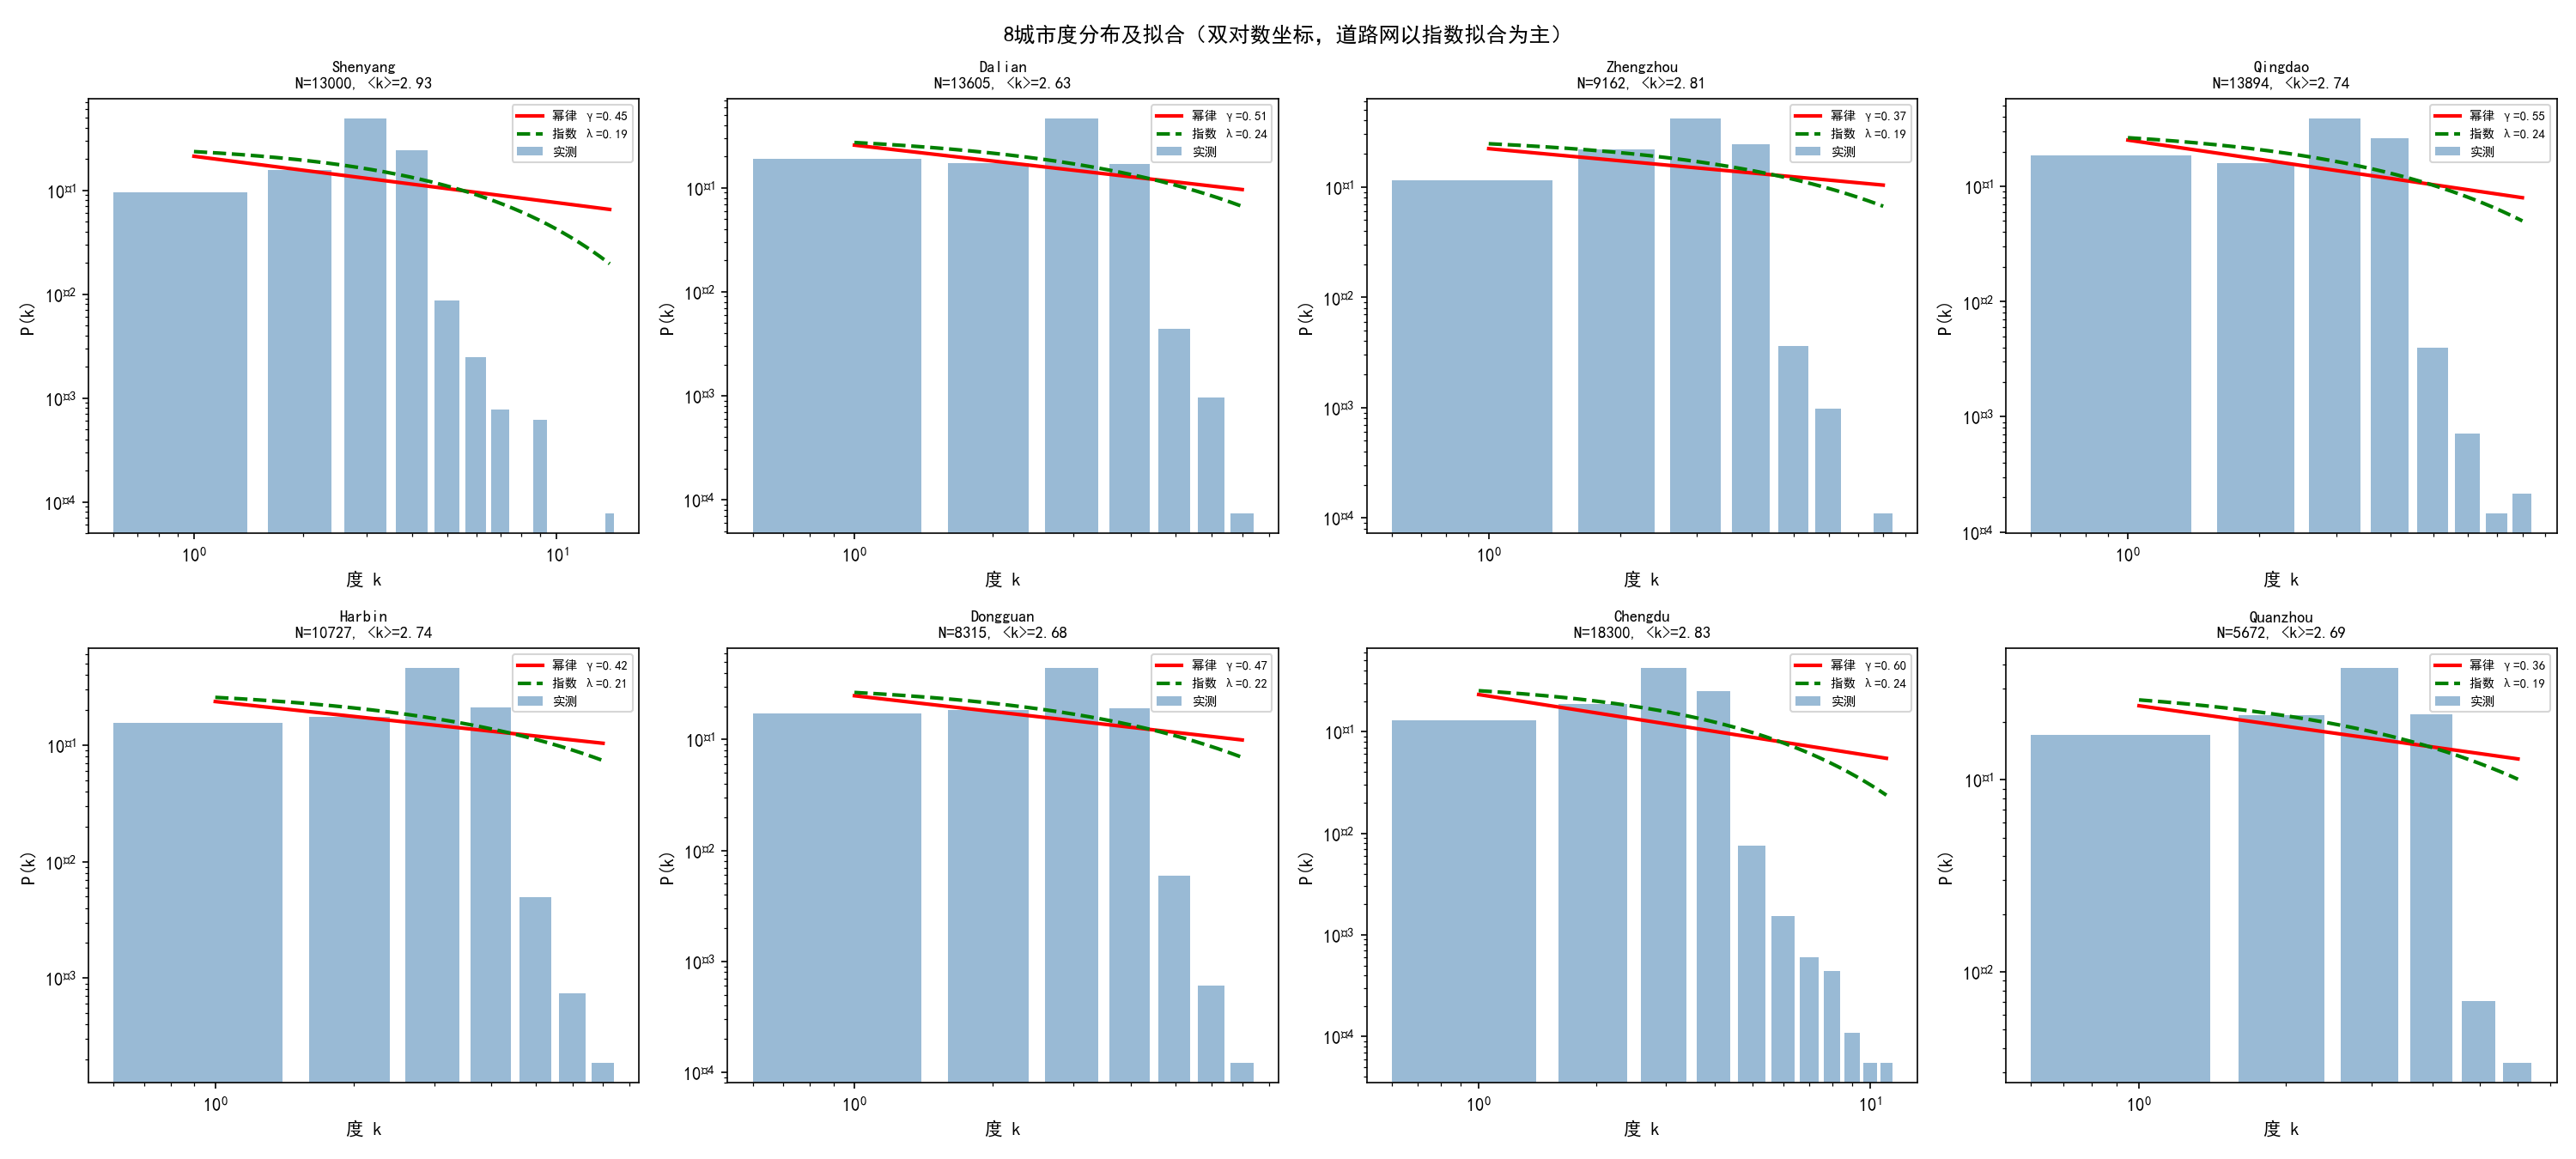
\includegraphics[width=\textwidth]{outputs/Q1_degree_distributions.png}
\caption{8个城市交通网络度分布及三种分布模型拟合结果（双对数坐标）}
\end{figure}

% ==================== 问题二 ====================
\subsection{问题二：随机节点故障健壮性分析}

\subsubsection{渗流理论框架}

在随机故障场景中，以概率$p$独立移除网络中的节点。定义网络连通性指标为最大连通分量与初始节点数之比$S(p) = |\text{LCC}(p)| / N_0$。\textbf{健壮性指标}定义为：
\begin{equation}
R = \int_0^1 S(p)\,dp
\end{equation}
该指标物理含义为：在节点随机移除过程中，网络维持连通性能力的累积度量。$R$越大，网络越健壮。

\subsubsection{Molloy-Reed理论渗流阈值}

根据Molloy-Reed准则~\cite{molloy1995critical}，对于具有给定度分布的随机图，巨连通分量消失的临界故障比例为：
\begin{equation}
f_c = 1 - \frac{1}{\kappa - 1}, \quad \kappa = \frac{\langle k^2 \rangle}{\langle k \rangle}
\end{equation}
其中$\langle k \rangle$和$\langle k^2 \rangle$分别为度的一阶矩和二阶矩。$\kappa$反映了度分布的异质性：$\kappa$越大，网络容忍随机故障的能力越强。

\subsubsection{蒙特卡罗模拟}

对每个城市进行10次独立随机节点移除模拟，每次以不同的随机种子生成移除序列。以1\%节点数为步长批量移除节点，记录$S(p)$曲线，取均值和标准差。同时标记三个关键点：
\begin{itemize}[leftmargin=2em]
    \item $p_{0.5}$：$S(p) \leq 0.5$的最小移除比例（50\%连通性丧失）
    \item $f_c$：Molloy-Reed理论阈值
    \item $p^*$：$|dS/dp|$最大处（网络最快崩溃点）
\end{itemize}

\subsubsection{结果与分析}

\begin{table}[H]
\centering
\caption{随机故障下8个城市的健壮性指标}
\begin{tabular}{lcccccc}
\toprule
\textbf{城市} & $R$ & $\sigma_R$ & $p_{0.5}$ & $f_c$(MR) & $p^*$ & $\kappa$ \\
\midrule
沈阳 & \textbf{0.2213} & 0.0056 & 0.234 & 0.551 & 0.288 & 3.228 \\
大连 & 0.1510 & 0.0061 & 0.154 & 0.502 & 0.158 & 3.006 \\
郑州 & 0.2068 & 0.0073 & 0.214 & 0.531 & 0.273 & 3.134 \\
青岛 & 0.1782 & 0.0088 & 0.186 & 0.535 & 0.215 & 3.150 \\
哈尔滨 & 0.1712 & 0.0042 & 0.165 & 0.522 & 0.252 & 3.094 \\
东莞 & 0.1799 & 0.0039 & 0.199 & 0.512 & 0.224 & 3.048 \\
成都 & 0.2051 & 0.0037 & 0.223 & 0.543 & 0.252 & 3.187 \\
泉州 & 0.1785 & 0.0063 & 0.183 & 0.521 & 0.225 & 3.088 \\
\bottomrule
\end{tabular}
\end{table}

\textbf{关键发现：}
\begin{itemize}[leftmargin=2em]
    \item \textbf{沈阳}在随机故障下健壮性最高（$R=0.2213$），这与其最高的平均度（$\langle k \rangle = 2.927$）和$\kappa$值（3.228）一致。
    \item \textbf{大连}健壮性最低（$R=0.1510$），仅15.4\%的节点失效即导致50\%连通性丧失。
    \item 理论渗流阈值$f_c$普遍高于实测$p_{0.5}$，这是因为$f_c$对应的是巨分量完全消失的阈值，而$p_{0.5}$仅要求LCC降至50\%。
    \item 蒙特卡罗模拟的标准差很小（$\sigma_R < 0.009$），表明随机故障结果具有良好的统计稳定性。
\end{itemize}

\begin{figure}[H]
\centering
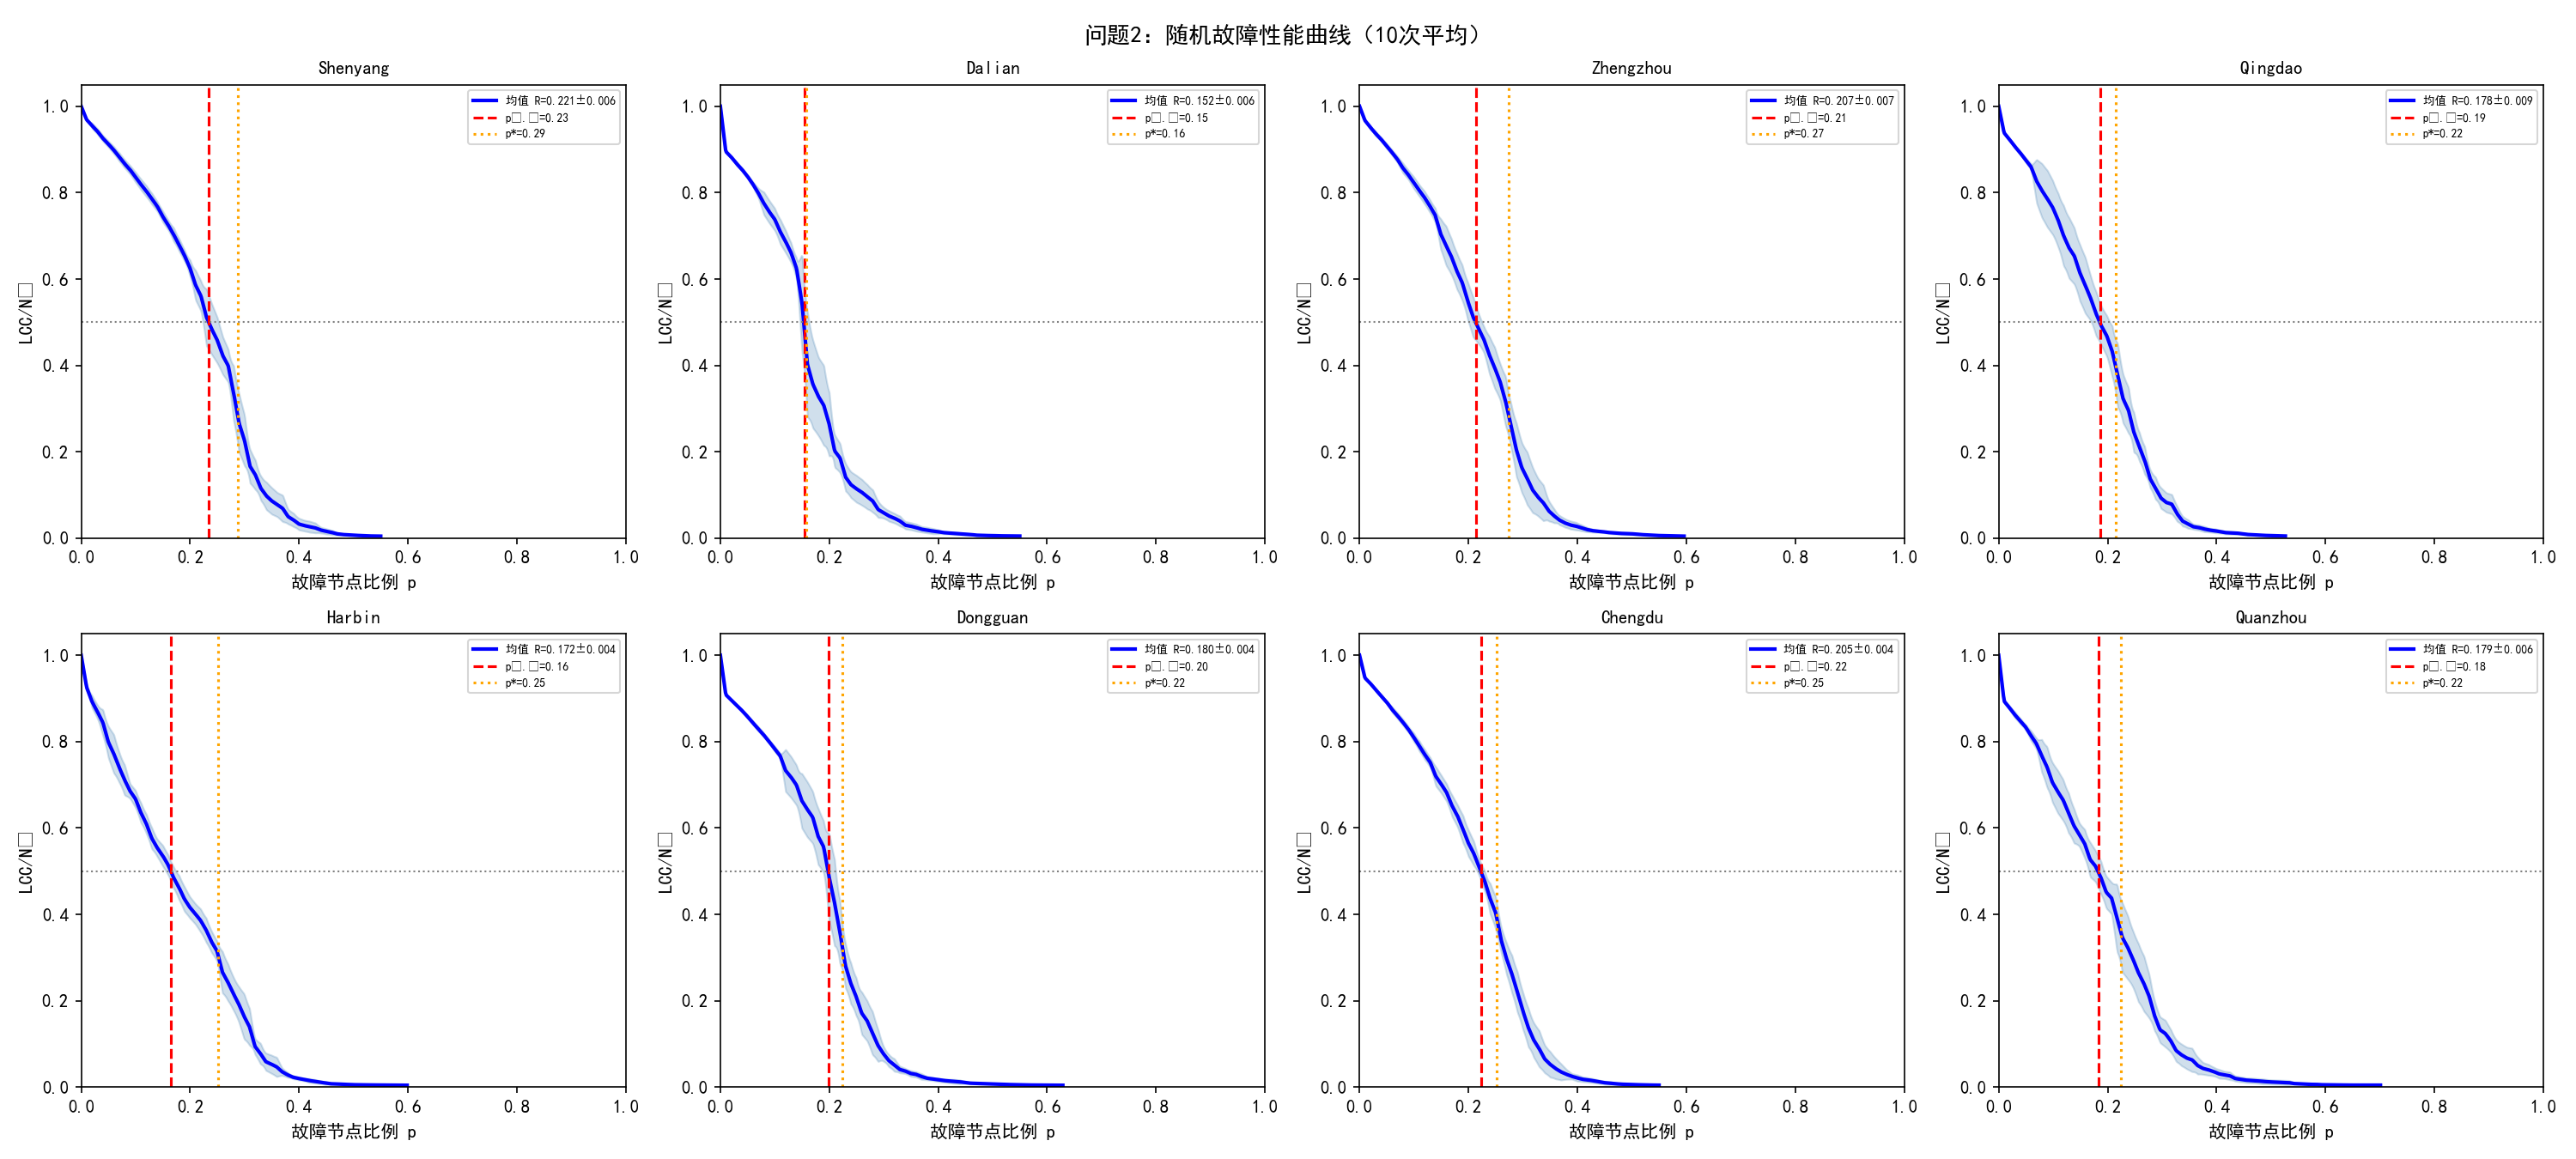
\includegraphics[width=\textwidth]{outputs/Q2_random_failure.png}
\caption{随机故障下8个城市的LCC$/N_0$演化曲线（10次均值$\pm$标准差，含Molloy-Reed理论阈值）}
\end{figure}

% ==================== 问题三 ====================
\subsection{问题三：最优蓄意攻击策略}

\subsubsection{攻击策略设计}

设计并比较三种节点移除策略：

\textbf{（1）自适应介数中心性攻击（HBA）}

HBA是已知最具破坏力的攻击策略之一~\cite{holme2002attack}。其核心思想是：每移除若干节点后重新计算剩余网络的介数中心性，始终优先移除当前介数最高的节点。介数中心性定义为：
\begin{equation}
B_C(v) = \sum_{s \neq v \neq t} \frac{\sigma_{st}(v)}{\sigma_{st}}
\end{equation}
其中$\sigma_{st}$是节点$s$到$t$的最短路径总数，$\sigma_{st}(v)$是经过$v$的最短路径数。

为平衡精度与计算效率，采用以下策略：
\begin{itemize}[leftmargin=2em]
    \item 近似介数：使用$k = \max(30, \min(150, N/60))$个采样节点估算
    \item 分批重算：每移除$N/25$个节点重新计算一次介数
\end{itemize}

\textbf{（2）静态度攻击}

按初始网络中节点度值降序排列一次性确定移除序列，不进行动态重算。

\textbf{（3）随机攻击}

作为基线对照，以随机顺序移除节点。

\subsubsection{健壮性曲线与指标}

对三种策略均计算$S(p)$曲线和健壮性积分$R$。同时记录HBA攻击下$S(p) \leq 0.01$时的移除比例，作为网络"实质瓦解"的标志。

\subsubsection{结果与分析}

\begin{table}[H]
\centering
\caption{三种攻击策略下的健壮性对比}
\resizebox{\textwidth}{!}{
\begin{tabular}{lccccccc}
\toprule
\textbf{城市} & $R_{\text{HBA}}$ & $R_{\text{度攻击}}$ & $R_{\text{随机}}$ & $\Delta R_{\text{HBA}}$ & $\Delta R_{\text{度}}$ & \textbf{HBA效力倍数} & $p$(LCC=1\%) \\
\midrule
沈阳 & \textbf{0.0972} & 0.1516 & 0.2175 & 0.1204 & 0.0659 & 5.5$\times$ & 0.400 \\
大连 & 0.0492 & 0.0978 & 0.1310 & 0.0818 & 0.0332 & 6.2$\times$ & 0.290 \\
郑州 & 0.0901 & 0.1544 & 0.2163 & 0.1262 & 0.0619 & 5.8$\times$ & 0.328 \\
青岛 & 0.0592 & 0.1470 & 0.1696 & 0.1104 & 0.0226 & 6.9$\times$ & 0.288 \\
哈尔滨 & 0.0756 & 0.1398 & 0.1741 & 0.0985 & 0.0343 & 5.3$\times$ & 0.329 \\
东莞 & 0.0727 & 0.1250 & 0.1912 & 0.1186 & 0.0663 & 6.3$\times$ & 0.369 \\
成都 & 0.0788 & 0.1408 & 0.1957 & 0.1168 & 0.0549 & 5.5$\times$ & 0.270 \\
泉州 & 0.0947 & 0.1457 & 0.1868 & 0.0921 & 0.0411 & 4.7$\times$ & 0.336 \\
\bottomrule
\end{tabular}
}
\end{table}

其中$\Delta R = R_{\text{随机}} - R_{\text{攻击}}$为攻击效力，HBA效力倍数$= \Delta R_{\text{HBA}} / \Delta R_{\text{度}}$。

\textbf{关键发现：}
\begin{itemize}[leftmargin=2em]
    \item HBA蓄意攻击下，\textbf{沈阳}健壮性最高（$R_{\text{HBA}} = 0.0972$），需移除40\%的节点才能使LCC降至1\%以下。
    \item \textbf{大连}在蓄意攻击下最为脆弱（$R_{\text{HBA}} = 0.0492$），仅需移除29\%的节点即可瓦解网络。
    \item HBA攻击效力比静态度攻击高1.8--4.9倍，比随机攻击高5--7倍，体现了动态重算的巨大优势。
    \item 所有城市在HBA攻击下的$R$值仅为随机故障下的35\%--45\%，说明蓄意攻击的破坏力远超随机故障。
\end{itemize}

\begin{figure}[H]
\centering
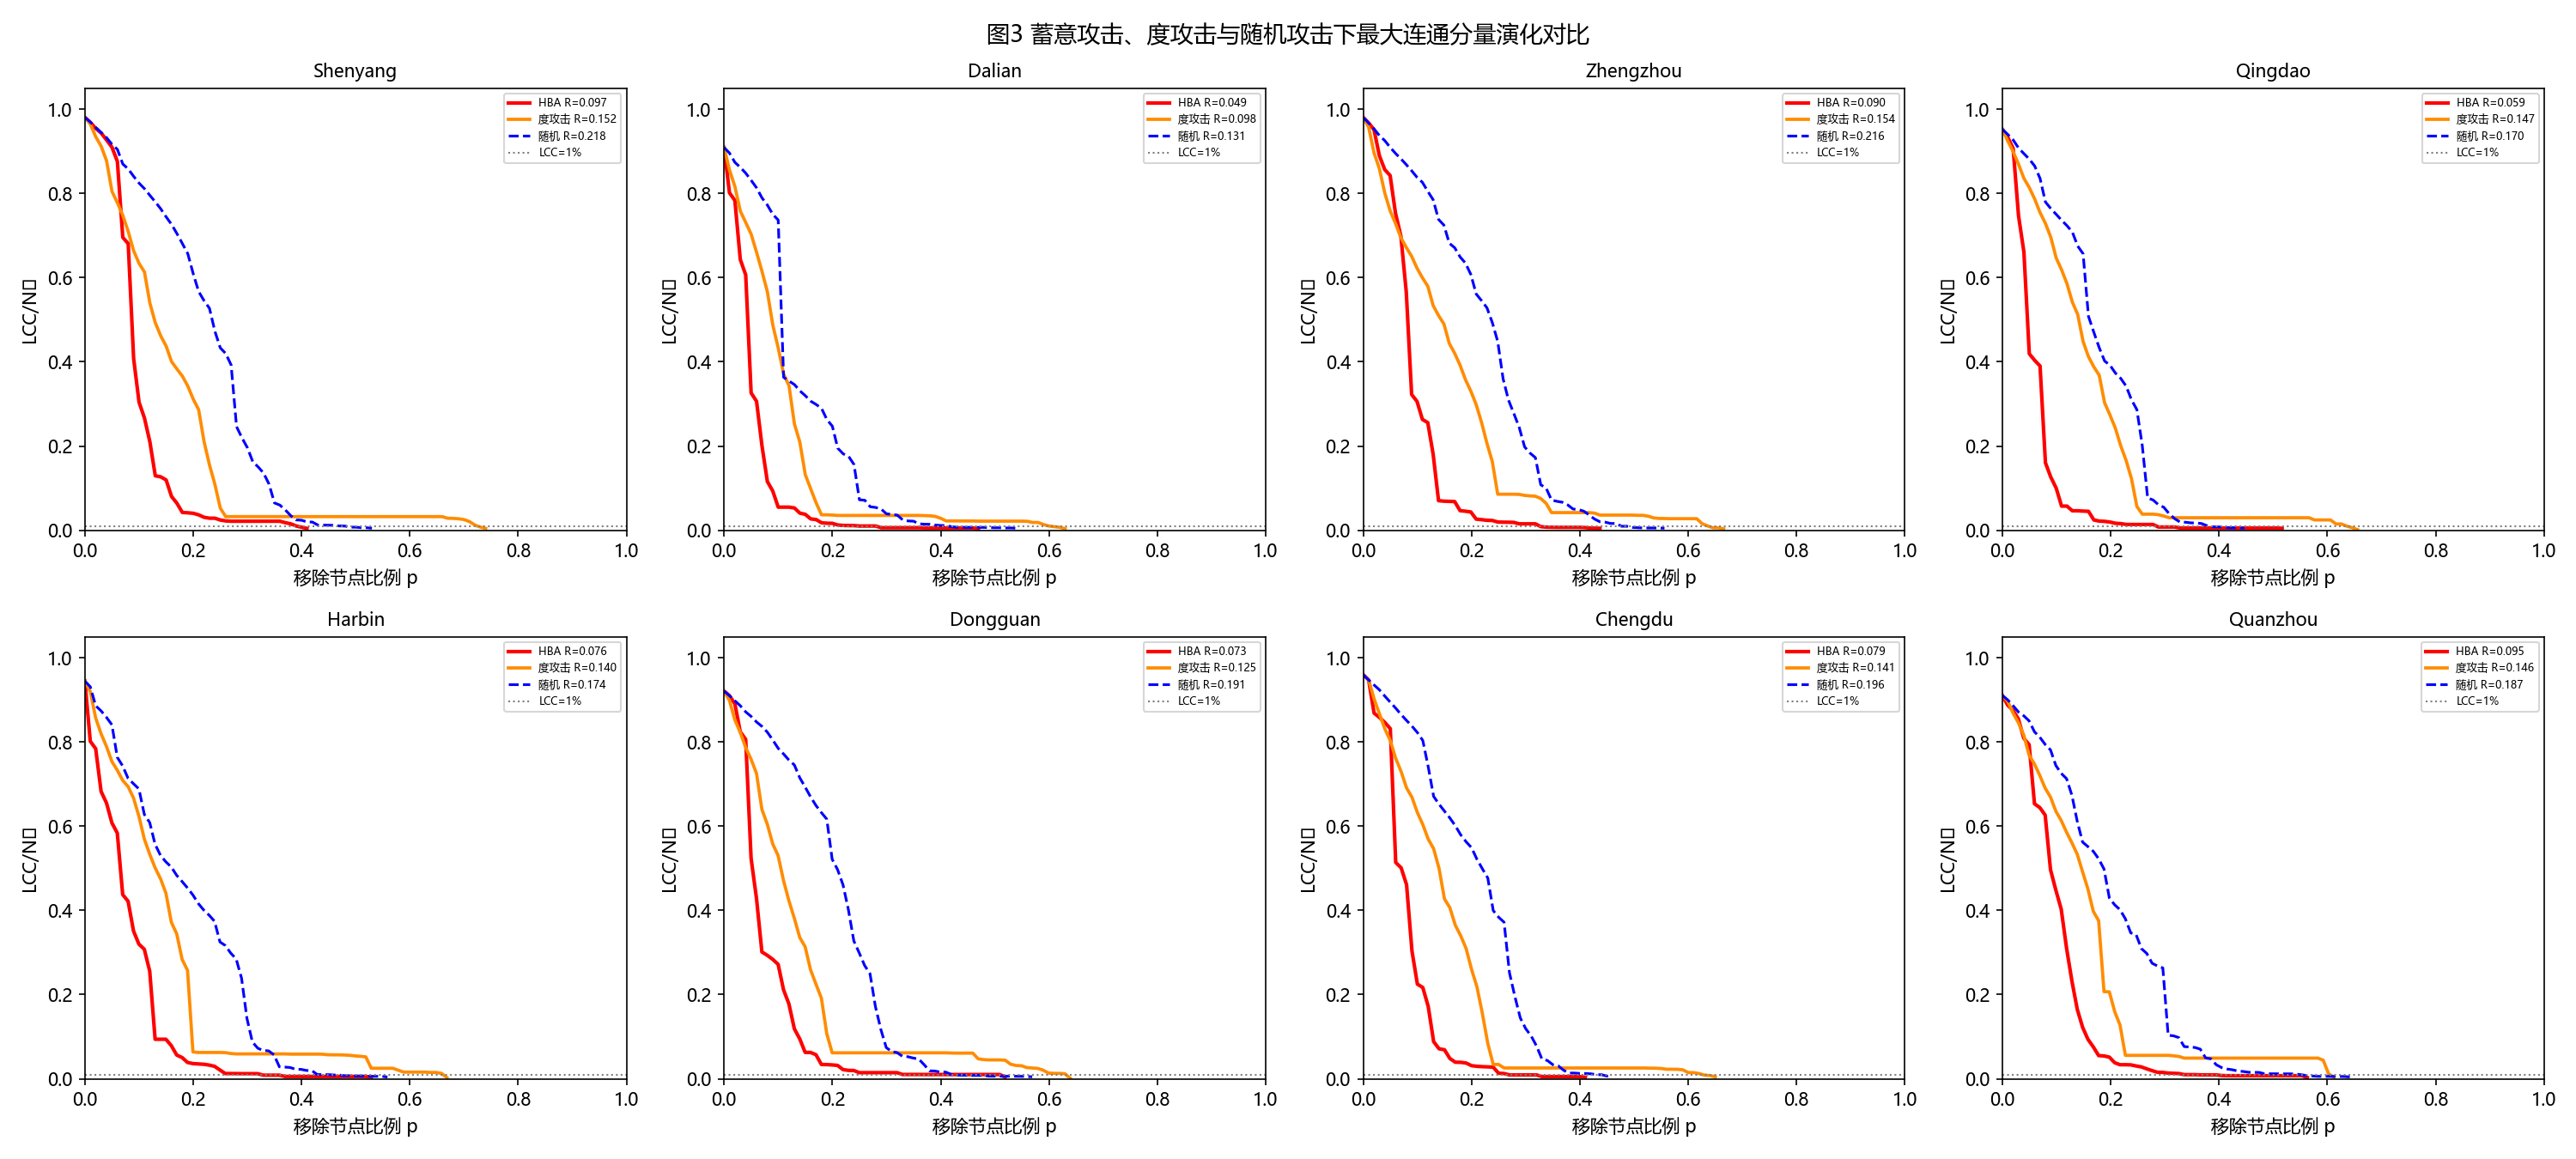
\includegraphics[width=\textwidth]{outputs/Q3_targeted_attack.png}
\caption{HBA蓄意攻击、度攻击与随机攻击下最大连通分量演化对比}
\end{figure}

% ==================== 问题四 ====================
\subsection{问题四：空间级联故障分析}

\subsubsection{空间级联模型}

在真实灾害场景中，某节点的失效往往会波及地理邻近的节点。定义空间级联故障模型如下：

\textbf{攻击过程：}每次选择当前存活节点中度最高的节点$v^*$作为攻击目标，同时移除以$v^*$为中心、半径$r$内的所有存活节点：
\begin{equation}
\text{Batch}(v^*) = \{u \in V_{\text{alive}} : \|u - v^*\| \leq r\}
\end{equation}
其中$\|\cdot\|$为欧氏距离。利用kd-tree数据结构实现$O(\log N)$的邻域查询。

\textbf{双视角分析：}
\begin{itemize}[leftmargin=2em]
    \item \textbf{节点比例视角}：以$p = \text{已移除节点数}/N_0$为x轴，反映网络在不同节点损失比例下的连通性。
    \item \textbf{攻击次数视角}：以攻击批次数为x轴，反映攻击者需要发动多少次攻击才能瓦解网络。
\end{itemize}

\subsubsection{实验设置}

对5种波及半径$r \in \{0, 500, 1000, 2000, 5000\}$米分别进行实验。$r=0$退化为逐节点攻击（与问题三的度攻击类似）。

\subsubsection{结果与分析}

\begin{table}[H]
\centering
\caption{不同波及半径下的空间级联故障健壮性$R$}
\begin{tabular}{lccccc}
\toprule
\textbf{城市} & $r=0$ & $r=500$m & $r=1000$m & $r=2000$m & $r=5000$m \\
\midrule
沈阳 & 0.1275 & 0.3813 & 0.4292 & 0.4618 & 0.4772 \\
大连 & 0.0871 & 0.3002 & 0.3418 & 0.3732 & 0.4031 \\
郑州 & 0.1214 & 0.3080 & 0.3772 & 0.4426 & 0.4601 \\
青岛 & 0.1066 & 0.3365 & 0.4017 & 0.4285 & 0.4602 \\
哈尔滨 & 0.1183 & 0.3106 & 0.3698 & 0.3856 & 0.4105 \\
东莞 & 0.1057 & 0.3206 & 0.3484 & 0.3600 & 0.3861 \\
成都 & 0.1097 & 0.3390 & 0.4020 & 0.4356 & 0.4228 \\
泉州 & 0.1025 & 0.2574 & 0.2669 & 0.3016 & 0.3645 \\
\bottomrule
\end{tabular}
\end{table}

\textbf{关键发现：}
\begin{itemize}[leftmargin=2em]
    \item 随着波及半径增大，以节点比例为x轴的健壮性$R$\textbf{反而增大}（$r=0$时$R \approx 0.10$，$r=5000$m时$R \approx 0.40$）。这一看似反直觉的结果可以解释为：大半径使每次攻击波及大量节点，降低了攻击的"精准性"——攻击者被迫同时移除许多非关键节点，"浪费"了攻击资源。
    \item 从攻击次数视角看，$r=5000$m时仅需44--130次攻击即可使LCC降至0.5\%以下，而$r=0$时需要1500--5200次。这说明空间级联极大地提高了攻击效率。
    \item 沈阳在所有半径下均保持最高或接近最高的健壮性，进一步验证了其网络的结构优势。
    \item 成都在$r=5000$m时$R$略有下降（0.4228 vs. $r=2000$m的0.4356），说明超大半径级联可能产生非单调效应。
\end{itemize}

\begin{figure}[H]
\centering
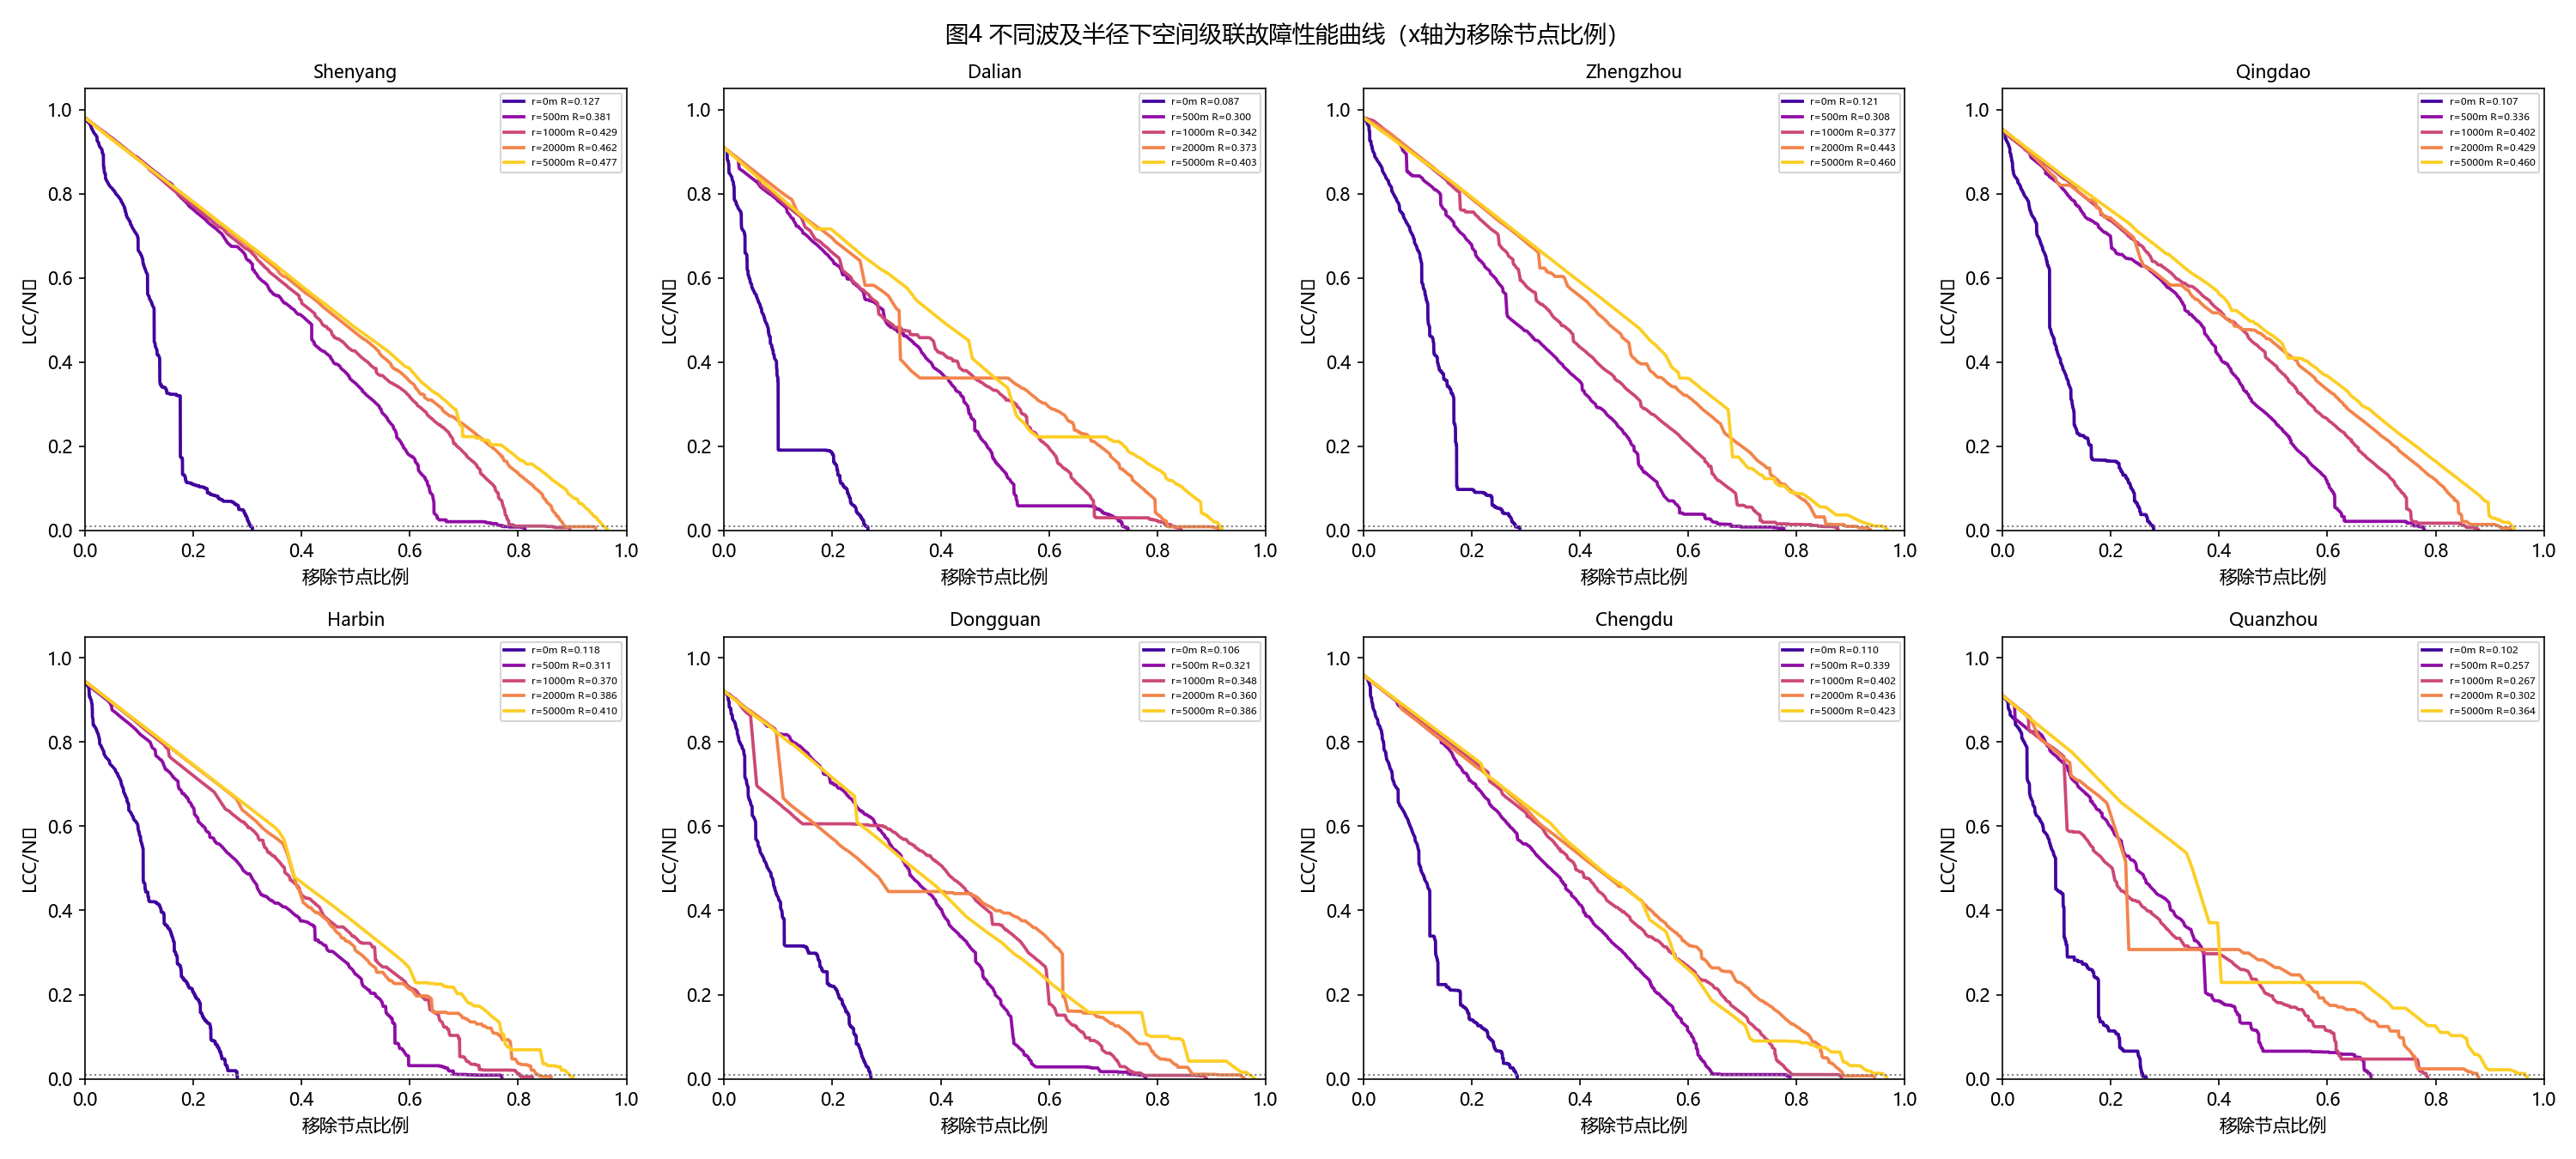
\includegraphics[width=\textwidth]{outputs/Q4_spatial_attack.png}
\caption{不同波及半径下空间级联故障的LCC$/N_0$演化曲线（x轴为移除节点比例）}
\end{figure}

% ==================== 问题五 ====================
\subsection{问题五：基于加边策略的网络健壮性提升}

\subsubsection{问题设定}

以问题三中健壮性最高的沈阳（$R_{\text{HBA}} = 0.0972$）为目标基准，为其余7个城市设计加边方案，使其HBA攻击健壮性达到或接近沈阳水平。建设成本定义为新增边的欧氏距离之和。

\subsubsection{候选边生成策略}

为克服$O(N^2)$候选空间的巨大搜索代价，设计两种启发式候选生成方法：

\textbf{策略一：桥边消除法}

桥边（bridge）是移除后会增加连通分量数的边。桥边的存在是网络脆弱性的直接来源。对每条桥边$(u,v)$，在$u$和$v$的邻居间生成替代连接，消除桥的关键性。候选按$\frac{B_C(u) + B_C(v)}{\text{cost}}$降序排列。

\textbf{策略二：介数旁路法}

针对介数中心性最高的$N/100$个节点（即最可能被HBA攻击的节点），在其邻居间建立"旁路"连接。具体地，对每个高介数节点$v$，选取其角度相对的邻居对$(u, w)$建立直连边，使得即使$v$被移除，$u$和$w$仍然连通。候选按$\frac{B_C(v)}{\text{cost}}$降序排列。

\subsubsection{贪心优化算法}

\begin{algorithm}[H]
\caption{贪心加边优化算法}
\begin{algorithmic}[1]
\REQUIRE 原始图$G$，目标健壮性$R_{\text{target}}$，预算$n_{\max}$
\ENSURE 加边列表，总成本
\STATE $G' \leftarrow G.\text{copy}()$
\STATE 初始化候选集 $\leftarrow$ 桥边候选 $\cup$ 介数旁路候选
\STATE $R_{\text{proxy}} \leftarrow$ \textsc{QuickR}($G'$) \COMMENT{快速健壮性估算}
\STATE 校准目标：$R'_{\text{target}} \leftarrow R_{\text{target}} \times (R_{\text{proxy}} / R_{\text{HBA\_baseline}})$
\FOR{$i = 1$ \TO $n_{\max}$}
    \IF{$R_{\text{proxy}} \geq R'_{\text{target}}$}
        \STATE \textbf{break}
    \ENDIF
    \STATE 从候选集中取性价比最高的未添加边$(u, w)$
    \STATE $G'.\text{add\_edge}(u, w)$
    \IF{$i \bmod 5 = 0$}
        \STATE $R_{\text{proxy}} \leftarrow$ \textsc{QuickR}($G'$)
    \ENDIF
\ENDFOR
\STATE $R_{\text{verified}} \leftarrow$ \textsc{HBA\_R}($G'$) \COMMENT{完整HBA验证}
\RETURN 加边列表，总成本，$R_{\text{verified}}$
\end{algorithmic}
\end{algorithm}

其中\textsc{QuickR}为基于静态介数排序的快速健壮性代理指标（步长2\%），计算速度约为完整HBA评估的1/10。通过线性校准（$\text{scale} = R_{\text{proxy\_init}} / R_{\text{HBA\_baseline}}$）将代理指标映射到HBA度量空间。

\subsubsection{结果与分析}

\begin{table}[H]
\centering
\caption{加边策略实施结果（预算200条边）}
\resizebox{\textwidth}{!}{
\begin{tabular}{lccccccl}
\toprule
\textbf{城市} & $R_{\text{HBA}}$(前) & $R_{\text{target}}$ & \textbf{新增边数} & \textbf{成本(km)} & $R_{\text{quick}}$(后) & $R_{\text{HBA}}$(后) & \textbf{状态} \\
\midrule
沈阳 & 0.0972 & 0.0972 & 0 & 0 & 0.0972 & 0.0972 & 目标城市 \\
大连 & 0.0492 & 0.0972 & 200 & 261.1 & 0.0684 & 0.0532 & 预算不足 \\
郑州 & 0.0901 & 0.0972 & 200 & 530.0 & 0.1261 & 0.0921 & 预算不足 \\
青岛 & 0.0592 & 0.0972 & 200 & 303.7 & 0.0821 & 0.0621 & 预算不足 \\
哈尔滨 & 0.0756 & 0.0972 & 200 & 780.9 & 0.1253 & 0.0787 & 预算不足 \\
东莞 & 0.0727 & 0.0972 & 200 & 280.9 & 0.0979 & 0.0710 & 预算不足 \\
成都 & 0.0788 & 0.0972 & 200 & 176.8 & 0.1309 & 0.0873 & 预算不足 \\
泉州 & 0.0947 & 0.0972 & 80 & 206.8 & 0.1298 & 0.0933 & 预算不足 \\
\bottomrule
\end{tabular}
}
\end{table}

\textbf{关键发现：}
\begin{itemize}[leftmargin=2em]
    \item \textbf{泉州}仅需80条新边（206.8 km）即基本接近目标（$R_{\text{HBA}}$从0.0947提升至0.0933，几乎达标）。
    \item \textbf{成都}在200条边内实现了最大的绝对提升（$R_{\text{HBA}}$从0.0788到0.0873，提升10.8\%），且总成本最低（176.8 km），性价比最高。
    \item \textbf{大连}和\textbf{青岛}即使投入200条边也仅实现约8\%和5\%的提升，说明其网络结构性缺陷较深，需要更大规模的改造。
    \item 代理指标$R_{\text{quick}}$系统性高于实际$R_{\text{HBA}}$（约1.3--1.5倍），线性校准有效但仍有偏差，表明代理指标在评估加边效果时的局限性。
    \item 成本差异显著：哈尔滨每条新增边平均3.9 km，成都仅0.88 km，反映了城市空间尺度和网络密度的差异。
\end{itemize}

\begin{figure}[H]
\centering
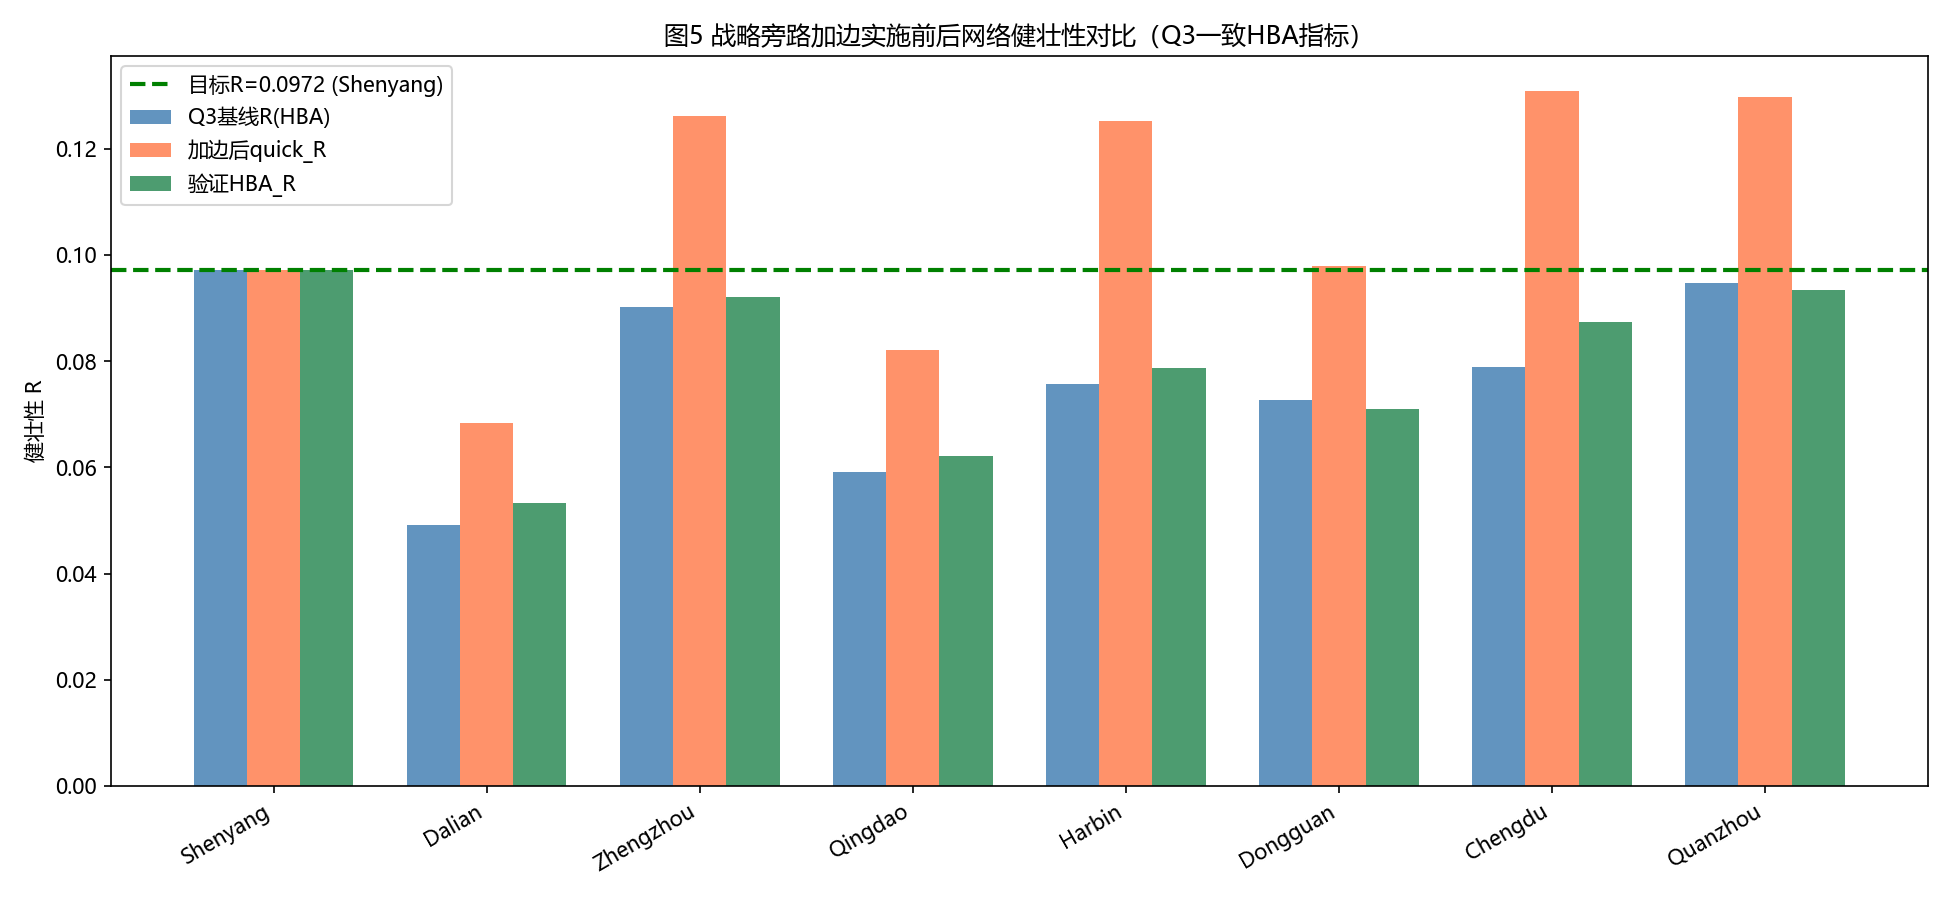
\includegraphics[width=\textwidth]{outputs/Q5_edge_addition.png}
\caption{加边策略实施前后各城市网络健壮性对比}
\end{figure}

% ==================== 五、模型评价 ====================
\section{模型评价与讨论}

\subsection{模型优点}

\begin{enumerate}[leftmargin=2em]
    \item \textbf{理论与实证相结合}：在随机故障分析中，Molloy-Reed理论渗流阈值与蒙特卡罗模拟互为验证，增强了结论的可信度。
    \item \textbf{多维度分析框架}：从随机故障、蓄意攻击、空间级联三个维度全面评估健壮性，揭示了不同场景下网络脆弱性的差异。
    \item \textbf{算法效率优化}：HBA攻击中采用近似介数和分批重算策略，在保持精度的同时将计算复杂度从$O(N^3)$降至可接受水平。加边优化中引入代理指标，避免了在每一步都运行完整HBA评估。
    \item \textbf{实际可操作性}：问题五的加边方案具体到每条新增边的端点和长度，可直接指导实际道路规划。
\end{enumerate}

\subsection{模型局限}

\begin{enumerate}[leftmargin=2em]
    \item \textbf{无向图简化}：实际交通网络包含单行道等有向结构，无向图建模可能高估连通性。
    \item \textbf{流量未建模}：健壮性仅从拓扑连通性角度衡量，未考虑道路容量、交通流量和拥堵效应。
    \item \textbf{加边策略的贪心性质}：贪心算法不保证全局最优，且代理指标与实际HBA健壮性存在系统偏差。
    \item \textbf{空间级联模型的同步性假设}：实际灾害中节点失效可能存在时序传播特征，而非瞬时同步失效。
\end{enumerate}

\subsection{改进方向}

\begin{itemize}[leftmargin=2em]
    \item 引入有向图和容量约束，建立更贴近实际的交通网络模型。
    \item 采用元启发式算法（如遗传算法、模拟退火）替代贪心策略进行加边优化。
    \item 在空间级联模型中引入时序传播机制（如SIR传播模型）。
    \item 结合实际交通流数据进行模型验证。
\end{itemize}

% ==================== 六、结论 ====================
\section{结论}

本文对8个中国城市的交通网络进行了系统的健壮性分析，主要结论如下：

\begin{enumerate}[leftmargin=2em]
    \item 8个城市的交通网络度分布均符合泊松分布而非幂律分布，表明其具有均匀随机网络特征。
    \item 在随机故障下，沈阳健壮性最高（$R=0.2213$），大连最低（$R=0.1510$）。
    \item 在HBA蓄意攻击下，沈阳仍为最健壮城市（$R_{\text{HBA}}=0.0972$），HBA攻击效力比随机攻击高5--7倍。
    \item 空间级联故障中，较大的波及半径反而提高了以节点比例衡量的健壮性$R$，但极大地减少了所需攻击次数。
    \item 基于桥边消除与介数旁路的贪心加边策略能有效提升网络健壮性，但对结构性缺陷较严重的城市（如大连），需要更大规模的网络改造。
\end{enumerate}

% ==================== 参考文献 ====================
\begin{thebibliography}{99}

\bibitem{molloy1995critical}
Molloy M, Reed B. A critical point for random graphs with a given degree sequence[J]. Random Structures \& Algorithms, 1995, 6(2-3): 161--180.

\bibitem{holme2002attack}
Holme P, Kim B J, Yoon C N, et al. Attack vulnerability of complex networks[J]. Physical Review E, 2002, 65(5): 056109.

\bibitem{albert2000error}
Albert R, Jeong H, Barab\'asi A L. Error and attack tolerance of complex networks[J]. Nature, 2000, 406(6794): 378--382.

\bibitem{callaway2000network}
Callaway D S, Newman M E J, Strogatz S H, et al. Network robustness and fragility: Percolation on random graphs[J]. Physical Review Letters, 2000, 85(25): 5468.

\bibitem{barabasi1999emergence}
Barab\'asi A L, Albert R. Emergence of scaling in random networks[J]. Science, 1999, 286(5439): 509--512.

\bibitem{newman2003structure}
Newman M E J. The structure and function of complex networks[J]. SIAM Review, 2003, 45(2): 167--256.

\bibitem{freeman1977set}
Freeman L C. A set of measures of centrality based on betweenness[J]. Sociometry, 1977, 40(1): 35--41.

\bibitem{brandes2001faster}
Brandes U. A faster algorithm for betweenness centrality[J]. Journal of Mathematical Sociology, 2001, 25(2): 163--177.

\bibitem{schneider2011mitigation}
Schneider C M, Moreira A A, Andrade Jr J S, et al. Mitigation of malicious attacks on networks[J]. Proceedings of the National Academy of Sciences, 2011, 108(10): 3838--3841.

\bibitem{boccaletti2006complex}
Boccaletti S, Latora V, Moreno Y, et al. Complex networks: Structure and dynamics[J]. Physics Reports, 2006, 424(4-5): 175--308.

\end{thebibliography}

\end{document}
